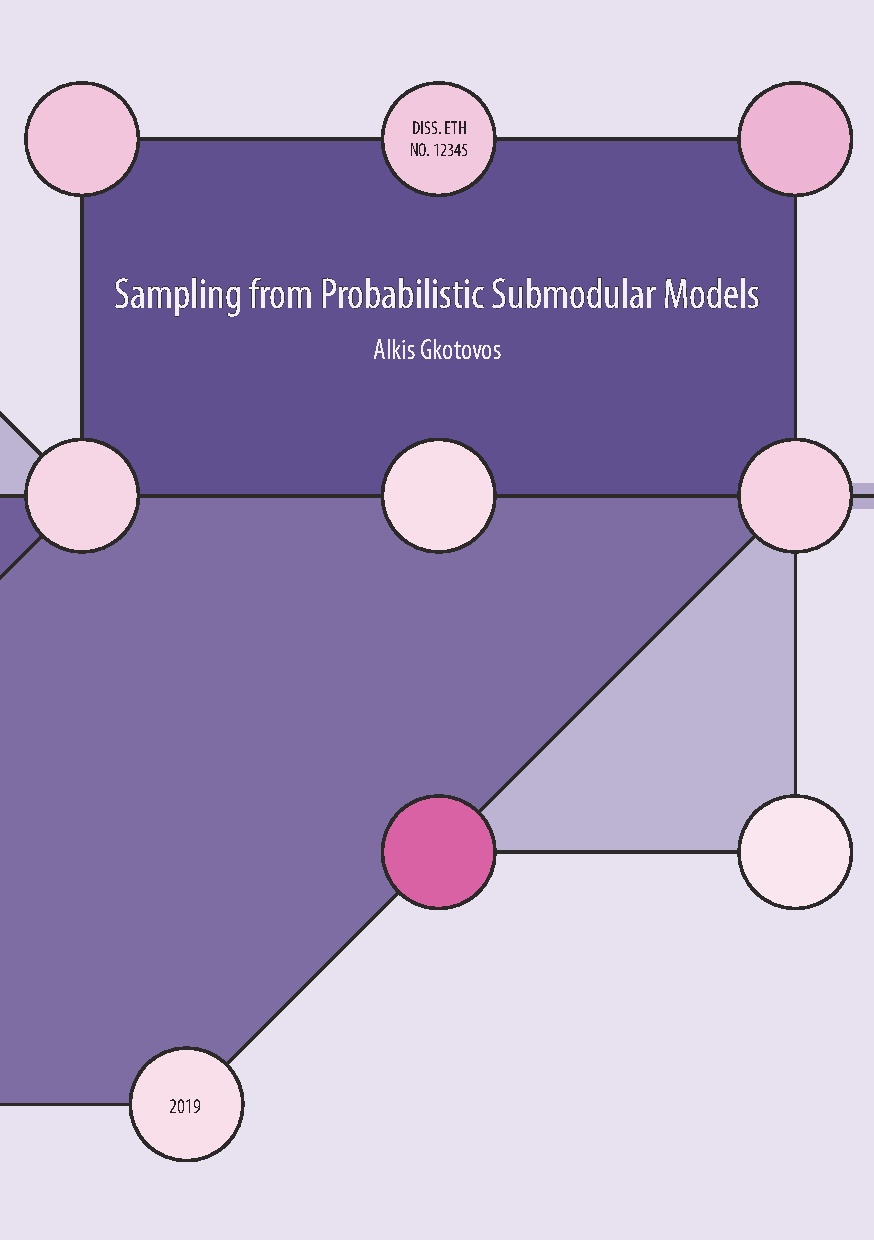
\includepdf[pages={1}]{title/outer.pdf}
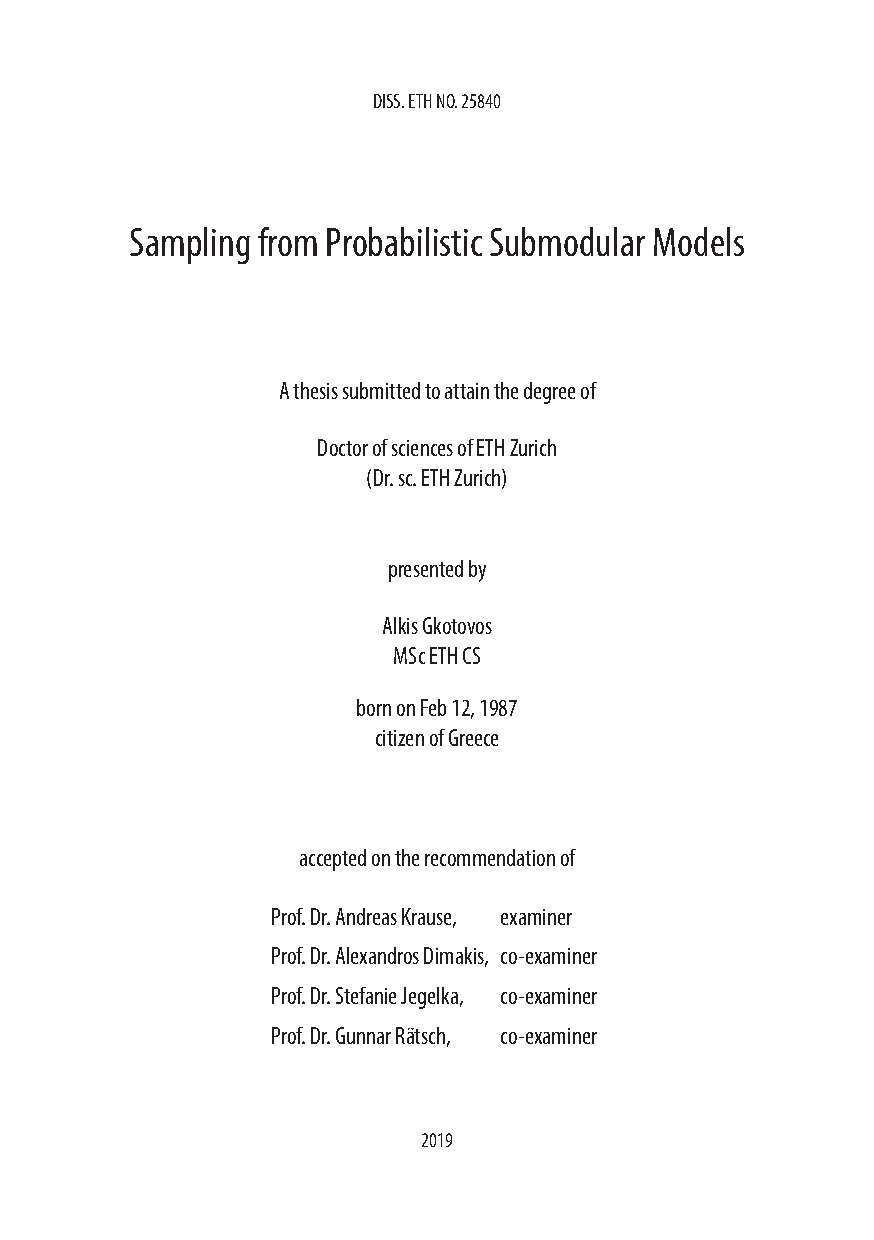
\includepdf[pages={1}]{title/inner.pdf}

\cleardoublepage
\section*{\centering Abstract}
\vspace{1em}
Practical problems of discrete nature are very common in machine learning; application domains include computer vision (e.g., image segmentation), sequential decision making (e.g., active learning), social network analysis (e.g., influence maximization), and natural language processing (e.g., document summarization).
Submodular set functions have found wide applicability in such problems for their ability to capture notions of coverage, diversity, or exclusivity; analogously, supermodular set functions have been used to capture notions of regularity, smoothness, or co-occurrence.

While the topic of submodular optimization has received much attention, these functions can also be used to define expressive discrete probabilistic models, called probabilistic submodular models.
Going beyond optimization, these models allow us to quantify predictive uncertainty, and suggest a maximum likelihood approach for learning such functions from noisy data.
Prominent examples of probabilistic submodular models include Ising and Potts models, as well as determinantal point processes, but the general class is much richer and little studied.

It is well known, though, that performing probabilistic inference in such models is computationally intractable in general.
In this thesis, we investigate the use of Markov chain Monte Carlo sampling as a means of performing approximate inference in probabilistic submodular models.

We start with analyzing the Gibbs sampler, and establish theoretical conditions that guarantee efficient convergence of this sampler in probabilistic submodular models.
We next propose a novel sampling procedure that makes use of discrete semigradients to perform efficient global moves, so as to avoid so-called state-space bottlenecks, and thus lead to improved convergence behavior.
Finally, we employ the aforementioned sampling methods to approximate the likelihood gradients, and learn such models from data.
We apply our learning procedure to the problem of modeling interactions between genetic mutations in cancer patients, and demonstrate considerable improvement over the state of the art in many of our experimental results on both synthetic and real cancer data.


\cleardoublepage
\begin{otherlanguage}{german}
\section*{\centering Zusammenfassung}
\vspace{1em}
Praktische Probleme diskreter Natur sind weit verbreitet im maschinellen Lernen.
Anwendungsbereiche umfassen unter anderen Computer Vision (z.B. Bildsegmentierung), sequentielle Entscheidungsfindung (z.B. aktives Lernen), soziale Netzwerkanalyse (z.B. Einflussmaximierung), und maschinelle Sprachverarbeitung (z.B. Dokumentzusammenfassung).
Submodulare Mengenfunktionen werden in diesen Bereichen häufig aufgrund ihrer Fähigkeit, Überdeckungsprobleme, Diversität oder Exklusivität zu modellieren, eingesetzt.
Analog werden Supermodulare Mengenfunktionen verwendet, um Regularität, Glattheit oder das gemeinsame Auftreten verschiedener Elemente zu modellieren.

Insbesondere der Themenbereich Submodulare Optimierung hat einige Aufmerksamkeit erregt, dabei können submodulare Funktionen ebenso der Definition diskreter probabilistischer Modelle dienen, auch bekannt unter dem Namen Probabilistische Submodulare Modelle.
Über ihre Optimierung hinaus ermöglichen sie uns auch, stochastische Unsicherheit zu quantifizieren und legen eine Maximum-Likelihood-Methode nahe, um sie auf Basis verrauschter Daten zu lernen.
Berühmte Beispiele Probabilistischer Submodularer Modelle sind vor allem Ising und Potts Modelle sowie Determinantal Point Processes.
Doch die generelle Modellklasse ist um einiges reichhaltiger und weniger gut untersucht. 

Allerdings ist allgemeint bekannt, dass die Inferenz dieser Modelle im Allgemeinen rechnerisch unmöglich ist.
Deshalb untersuchen wir in dieser Dissertation die Markov-Ketten-Monte-Carlo (MCMC) Verfahren zur approximativen Inferenz Probabilistischer Submodularer Modelle.

Zunächst analysieren wir Gibbs Sampling und etablieren theoretische Voraussetzungen, unter denen dieser Algorithmus bei Probabilistischen Submodularen Modellen effizient konvergiert.
Als nächstes stellen wir ein neuartiges Verfahren zur Stichprobenentnahme vor, die diskrete Halbgradienten gebraucht, um effiziente globale Schritte zu unternehmen.
Dies vermeidet sogenannte Zustandsraumengpässe (bottlenecks) und führt zu verbessertem Konvergenzverhalten.
Letztendlich benutzen wir zuvor erwähnte Sampling Methoden, um Likelihood-Gradienten zu approximieren und unsere Modelle aus Daten zu lernen.
Konkret verwenden wir unser Lernverfahren, um die Interaktionen genetischer Mutationen in Krebspatienten zu modellieren.
Sowohl für synthetische als auch echte Daten erzielen wir erhebliche Verbesserungen in vielen unserer Experimente im Vergleich zum neuesten Stand der Forschung.
\end{otherlanguage}

\cleardoublepage
\section*{\centering Acknowledgements}
\vspace{1em}